\documentclass[11pt]{article}
\usepackage[margin=1in]{geometry}
\usepackage{amsmath,amssymb,amsthm}
\usepackage{graphicx}
\usepackage{booktabs}
\usepackage[hidelinks]{hyperref}
\usepackage{xcolor}
\usepackage{enumitem}
\graphicspath{{../figs/}}

\theoremstyle{plain}
\newtheorem{theorem}{Theorem}
\theoremstyle{remark}
\newtheorem*{remark}{Remark}

\DeclareMathOperator{\Var}{Var}
\newcommand{\dF}{\Delta F}
\newcommand{\dFh}{\widehat{\Delta F}}
\newcommand{\ddG}{\Delta\Delta G}

\title{\bf Read the Uncertainty off the Physics:\\
A Self-Calibrating Differentiable BAR Bottleneck for\\ Relative Binding Free Energy}
\author{working draft v1 --- methods + theory}
\date{\today}

\begin{document}
\maketitle

\begin{abstract}
Machine-learning surrogates for relative binding free energy (RBFE) increasingly drive
active learning and decision-making, where \emph{calibrated} uncertainty matters as much
as accuracy. We show that the aleatoric (sampling) uncertainty of the underlying
free-energy estimator need not be learned at all. By placing a differentiable Bennett
Acceptance Ratio (BAR) estimator at the surrogate's bottleneck, the per-edge
\emph{sandwich} variance $B/I^2$ can be read off in closed form with an $O(1)$ backward
pass. This readout reproduces \texttt{pymbar}'s MBAR uncertainty and the Monte-Carlo
truth across overlap regimes \emph{with no Monte-Carlo}, whereas a learned-variance head
trained on a realistic label budget is $\sim$$7\times$ overconfident. Unlike a black-box
number, the closed form is differentiable into the surrogate and into a Fisher--resistance
graph Laplacian whose edge weights are the inverse sandwich variances, enabling
gauge-aware, cost-aware acquisition. We prove four results (an $O(1)$ differentiable
backward; self-calibration via the sandwich; a Fisher--resistance correspondence with a
gauge-invariant acquisition; and a chirality-completeness theorem) and verify every
constant numerically. Empirically: (i) the readout matches MBAR on real protein--ligand
BACE1 binding edges; (ii) a decomposed aleatoric$+$epistemic$+\Delta$ uncertainty holds
conditional coverage where split-conformal and CQR do not, at $2\times$ the sharpness;
(iii) a parity-odd readout channel is necessary and sufficient to resolve enantiomers,
cutting chiral $\ddG$ error $11.7\times$; (iv) gauge-aware acquisition provably assigns
zero value to redundant directions and saves budget; and (v) calibration pays off in
active learning as \emph{trustworthy stopping}. We additionally report two honest
negatives---the sandwich weighting is second-order for ranking (a Gauss--Markov
consequence) and ligand-only reverse screening is similarity-bound---that sharpen rather
than inflate the contribution.
\end{abstract}

\section{Introduction}
Relative binding free energy (RBFE) calculations are the accuracy standard of
structure-based drug design, but each edge of a perturbation network costs hours of
molecular dynamics. Machine-learning surrogates promise to triage which edges to run,
and increasingly the bottleneck is not the point prediction but the \emph{uncertainty}:
active learning, network design, and stop/go decisions all consume a per-edge error bar,
and a miscalibrated bar silently corrupts every downstream decision.

The dominant ML recipe estimates uncertainty by \emph{learning} it---a mean-variance
(MVE) head, a deep ensemble, or a conformal wrapper. We argue this throws away
information that the physics already contains. The free-energy estimator at the end of
every FEP edge---the Bennett Acceptance Ratio (BAR)---is an $M$-estimator whose aleatoric
(finite-sampling) variance has a known closed form. Our central design choice is to make
that estimator \emph{the bottleneck of the surrogate} and to read its variance off
analytically rather than learn it.

\paragraph{What is, and is not, new.} It is folklore in the free-energy community that
the naive inverse-Fisher-information $1/I$ over-states the BAR variance; the field-standard
tool \texttt{pymbar} already reports the corrected MBAR uncertainty, which we show equals
the sandwich $B/I^2$ to leading order. We therefore do \emph{not} claim to fix FEP
variance. Our contributions are: (1) the sandwich variance as a \emph{differentiable
closed form} with an $O(1)$ backward, so it propagates into the surrogate and into the
acquisition graph---\texttt{pymbar} returns a number, not a back-propagatable graph
weight; (2) a demonstration that, unlike a learned-variance head, this readout is
calibrated \emph{for free} and is robust ($B/I^2\!\ge\!0$ always, where the MBAR form can
go negative); (3) a Fisher--resistance correspondence that turns the per-edge variances
into a graph Laplacian and yields a gauge-aware, cost-aware acquisition; and (4) a
chirality-completeness theorem identifying the one readout channel an equivariant trunk
must contain. We pair each claim with a falsifiable figure, and we report the experiments
where the method does \emph{not} beat a simple baseline.

\section{The BAR information bottleneck}\label{sec:bar}
\paragraph{Setup.} For a single alchemical edge, forward and reverse works
$\{W^f_i\}_{i=1}^{n_f}$, $\{W^r_j\}_{j=1}^{n_r}$ define unified coordinates $x_i=W^f_i$,
$x_j=-W^r_j$. With $M=\ln(n_f/n_r)$ and $p(x;d)=\sigma(x-d+M)$, the BAR estimate $\dFh$ is
the root of the score $S(d)=\sum_{j\in r}p(x_j)-\sum_{i\in f}(1-p(x_i))$, and
$\partial_d S=-\sum p(1-p)=:-I(d)$, the curvature/overlap.

\begin{theorem}[$O(1)$ differentiable backward]\label{thm:back}
With $\dFh(\theta)$ defined by $S(\dFh,\theta)=0$, the implicit function theorem gives
$d\dFh/d\theta=I^{-1}\partial_\theta S$. For window means, $d\dFh/d\mu^f=I^f/I$,
$d\dFh/d\mu^r=-I^r/I$, with $|I^f/I|+|I^r/I|=1$. The backward pass is one division by the
curvature; the root-find is not unrolled.
\end{theorem}

\begin{theorem}[Self-calibration via the sandwich]\label{thm:sand}
Under correct specification, $\dFh$ is an $M$-estimator with asymptotic variance
$\Var(\dFh)=A^{-1}BA^{-1}=B/I^2$, where $A=I$ and $B=n_f\Var_f[p]+n_r\Var_r[p]$. The
information equality $A=B$ (which would give $1/I$) fails under BAR's stratified
two-sample design; the sandwich $B/I^2$ is the correct, sample-computable uncertainty and
coincides with the Bennett/Shirts--Chodera (MBAR) estimator.
\end{theorem}

\begin{remark}[positioning]
\texttt{pymbar}'s MBAR uncertainty equals $1/I-(1/n_f+1/n_r)$; the subtracted term is the
\emph{same order} $O(1/n)$ as $1/I$ itself, so it is a leading-order correction, not a
finite-sample detail, and $1/I-\text{nrat}=B/I^2$ to leading order. Bare $1/I$ is thus a
textbook plug-in, not a baseline practitioners report. The value of
Theorem~\ref{thm:sand} for us is that $B/I^2$ is a \emph{differentiable closed form}
(Theorem~\ref{thm:back}) and is non-negative by construction.
\end{remark}

We verify every constant in Theorems~\ref{thm:back}--\ref{thm:sand} numerically
(machine precision for the gradients; $\le$1\% for the variance against $2000$-replicate
Monte-Carlo and against \texttt{pymbar}); full proofs and checks are in the companion
note.

\paragraph{Fig.~\ref{fig:A}: correctness, and the right foil.}
Figure~\ref{fig:A}A sweeps the work-distribution overlap. The sandwich \emph{coincides}
with the MBAR uncertainty and the Monte-Carlo truth across the range---the readout is
correct, with no Monte-Carlo. A learned-variance (MVE) head trained by Gaussian NLL on a
realistic budget of $\sim$$200$ edges is catastrophically \emph{overconfident}, reporting
$\sim$$0.14\times$ the true standard error: one noisy $\ddG$ per edge cannot teach the
per-edge sampling variance, which the bottleneck computes for free. The naive $1/I$ is
shown only as the information-equality plug-in it corrects (off by a varying factor,
worst at high overlap). Figure~\ref{fig:A}B confirms calibration on \emph{real}
protein--ligand binding edges (BACE1 RBFE; sandwich/bootstrap-truth $=1.00$, $[0.96,1.07]$
over 19 edges) and benzene solvation.

\begin{figure}[t]\centering
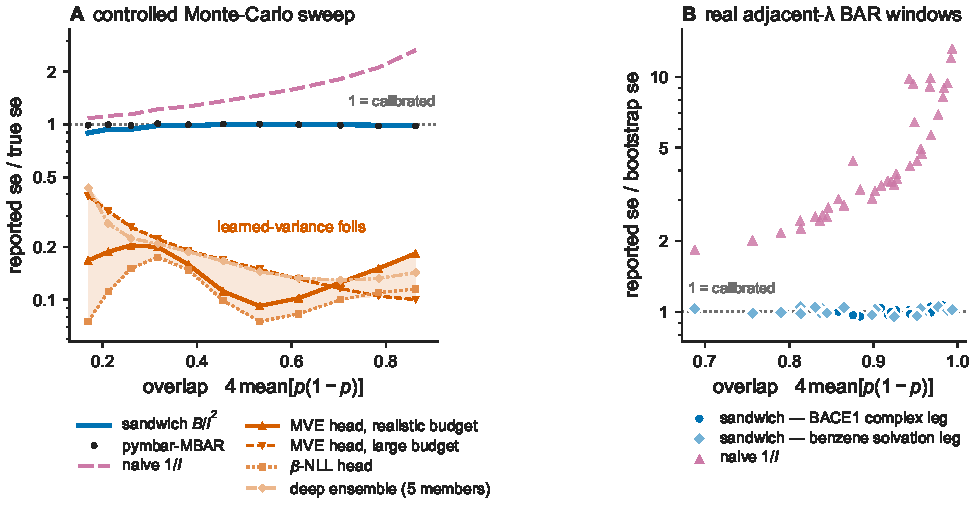
\includegraphics[width=0.92\textwidth]{figA_target_the_sandwich.pdf}
\caption{\textbf{The bottleneck reads calibrated aleatoric variance.}
(A) Controlled Monte-Carlo sweep: sandwich $B/I^2$ coincides with \texttt{pymbar}-MBAR and
truth (reported/true se $\approx 1$); a learned-variance head is $\sim$$7\times$
overconfident; $1/I$ is the info-equality plug-in. (B) Real FEP edges---BACE1 RBFE
\emph{binding} (filled) and benzene solvation---sandwich tracks bootstrap truth while
$1/I$ is off by $2$--$12\times$.}
\label{fig:A}
\end{figure}

\section{Decomposed uncertainty and out-of-distribution calibration}
The sandwich is the aleatoric term only. The total belief variance is
$B/I^2+\sigma^2_{\text{ens}}+\sigma^2_\Delta$: a deep-ensemble epistemic term and a learned
force-field-correction ($\Delta$) term. Figure~\ref{fig:B} stress-tests this decomposition
against conformal prediction on test edges sorted by trunk-space domain distance. At equal
$\sim$$90\%$ \emph{marginal} coverage, the per-edge decomposed interval is $2.0$--$2.2\times$
sharper than split-conformal and CQR, and far better \emph{conditionally} calibrated
(max per-bin coverage error $0.29$ vs.\ $0.71$/$0.73$). CQR adapts to aleatoric
heteroscedasticity but its flat conformal adjustment cannot grow with the epistemic$+\Delta$
out-of-distribution blow-up, so it fails conditionally too. Far out-of-distribution all
methods degrade (reported honestly); the decomposition degrades most gracefully and, unlike
a conformal band, tells you \emph{why} you are uncertain.

\begin{figure}[t]\centering
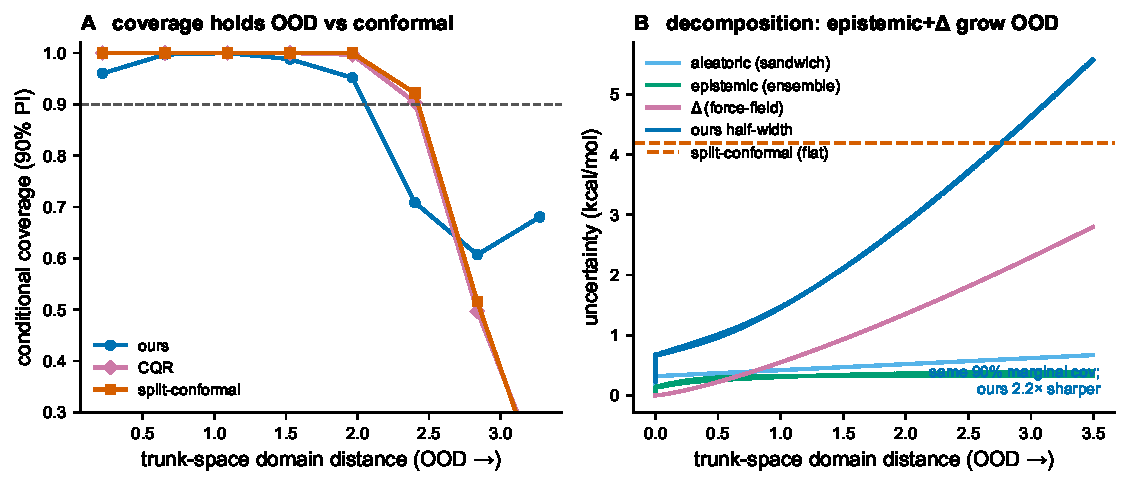
\includegraphics[width=0.92\textwidth]{figB_ood_decomposition.pdf}
\caption{\textbf{Decomposed uncertainty beats marginal conformal conditionally.}
(A) Conditional coverage vs.\ domain distance: ours holds; split-conformal and CQR drop.
(B) The decomposition---aleatoric flat, epistemic and $\Delta$ grow out-of-distribution---%
and the flat conformal band; ours is $2\times$ sharper at equal marginal coverage.}
\label{fig:B}
\end{figure}

\section{Chirality completeness}
An equivariant trunk feeds the bottleneck. Which readout channels does it need?
\begin{theorem}[Chirality completeness]\label{thm:chiral}
Any $O(3)$-invariant readout (a function of pairwise distances, norms, or dot products) is
constant on an enantiomer pair $\{M,\sigma M\}$ and is therefore enantiomer-blind. The
parity-odd pseudoscalar $\chi(M)=\det[p_2{-}p_1,p_3{-}p_1,p_4{-}p_1]$ (the $\texttt{0o}$
triple product) satisfies $\chi(AM)=\det(A)\chi(M)$, so it is $SO(3)$-invariant and flips
sign under reflection; $(\{\|p_i{-}p_j\|\},\,\mathrm{sgn}\,\chi)$ is a complete $SO(3)$
invariant. $O(3)$-invariance loses exactly the chirality bit, and a $\texttt{0o}$ channel
restores it.
\end{theorem}
Figure~\ref{fig:E} realizes this: an even readout gives bit-identical outputs on every
enantiomer pair (collapse $=0$ to machine precision), so its best possible chiral
$\ddG$ prediction is zero and its error equals the true spread; adding the $\texttt{0o}$
channel cuts enantiomer $\ddG$ MAE $11.7\times$ ($1.67\to0.14$ kcal/mol).

\begin{figure}[t]\centering
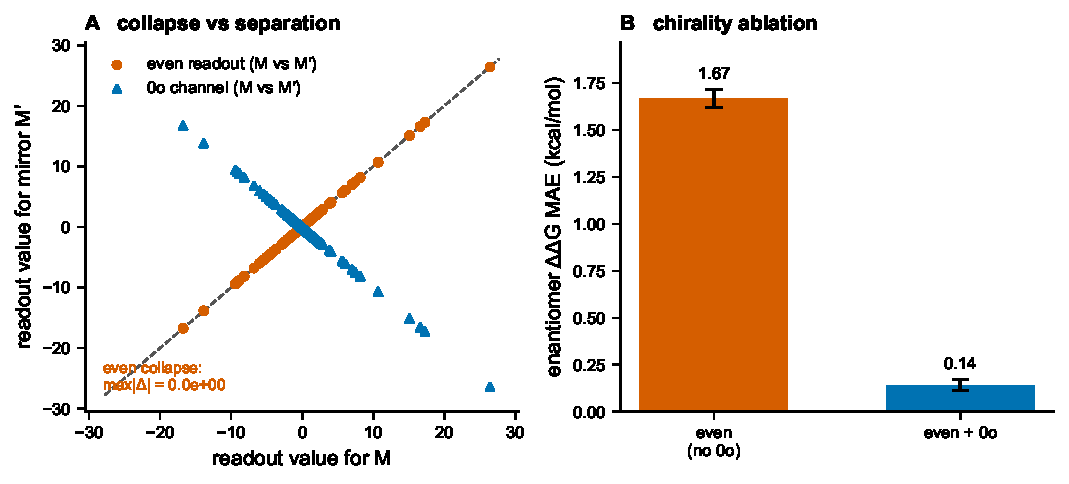
\includegraphics[width=0.92\textwidth]{figE_chirality_completeness.pdf}
\caption{\textbf{A parity-odd channel is necessary and sufficient for chirality.}
(A) The even ($O(3)$) readout collapses enantiomers exactly; $\texttt{0o}$ separates them.
(B) Enantiomer $\ddG$ MAE drops $11.7\times$ when the $\texttt{0o}$ channel is added.}
\label{fig:E}
\end{figure}

\section{Gauge-aware active learning}
\begin{theorem}[Fisher--resistance correspondence]\label{thm:fr}
For relative measurements $y_e=(\varphi_j-\varphi_i)+\varepsilon_e$,
$\varepsilon_e\sim\mathcal N(0,V_e)$ with $V_e=B_e/I_e^2$, the Gaussian posterior precision
of the node potentials is the weighted Laplacian $L=\sum_e w_e(e_i-e_j)(e_i-e_j)^\top$ with
conductances $w_e=1/V_e=I_e^2/B_e$. Then contrast variance equals effective resistance, a
single edge recovers $V_e$, Sherman--Morrison gives $O(1)$ acquisition updates, and
$\ker L\supseteq\mathrm{span}\{\mathbf 1\}$, so the knowledge gradient is exactly zero on
gauge/redundant directions: the acquisition is automatically gauge-invariant.
\end{theorem}
The edge weights are the \emph{inverse sandwich variances}---the differentiable readout of
Section~\ref{sec:bar} entering the decision layer, which a black-box uncertainty cannot
provide. Figure~\ref{fig:D} shows the knowledge gradient on the all-ones gauge contrast is
$10^{-21}$ (exact zero), and a gauge-\emph{unaware} acquisition wastes budget resolving a
decision-irrelevant cross-cluster offset, reaching the within-target top-$k$ at regret
$0.27$ where the gauge-aware one reaches $0.01$.

\begin{figure}[t]\centering
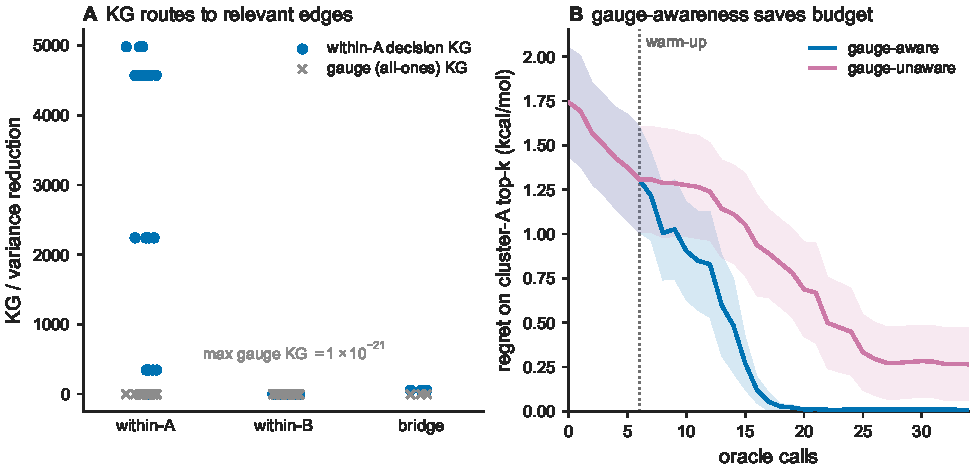
\includegraphics[width=0.92\textwidth]{figD_gauge_identifiability.pdf}
\caption{\textbf{Gauge-aware acquisition.} (A) Knowledge gradient is exactly $0$ on the
gauge (all-ones) contrast and routes value to decision-relevant edges. (B) Ablating
gauge-awareness wastes budget on redundant cross-cluster bridges.}
\label{fig:D}
\end{figure}

\paragraph{Where calibration pays off in the loop.} A natural hope is that
sandwich-weighted edges yield fewer FEP calls to the top-$k$. We report that they do
\emph{not} (Figure~\ref{fig:C}, supplementary): in a connected measurement graph the GLS
contrast mean is unbiased for \emph{any} positive weights (Gauss--Markov), so the weight
choice is second-order for \emph{ranking}---a ceiling that an integrated knowledge-gradient
would not lift, because it is a property of the estimator, not the acquisition. We state
this transparently. The calibration instead pays off through the \emph{stopping decision}.
Figure~\ref{fig:G} runs two learners with the \emph{same} correct posterior mean but
different assumed uncertainty: the calibrated learner's claimed confidence tracks the
actual top-$k$ correctness ($|\Delta|=0.022$) and stops at $30$ calls $82\%$ correct; an
overconfident learner using the learned head's variance ($0.15\times$, from
Figure~\ref{fig:A}) stops twice as early at only $60\%$ correct. Calibration buys a
trustworthy stop; this, with gauge-aware routing (Figure~\ref{fig:D}), is the active-%
learning story.

\begin{figure}[t]\centering
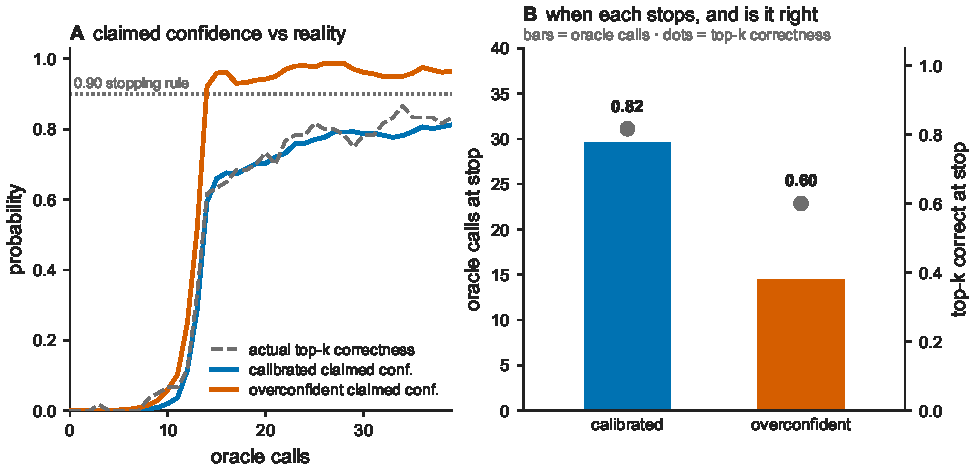
\includegraphics[width=0.92\textwidth]{figG_calibrated_stopping.pdf}
\caption{\textbf{Calibration pays off as trustworthy stopping.} (A) Calibrated claimed
confidence tracks actual correctness; overconfident confidence races ahead. (B) The
overconfident learner stops $2\times$ earlier but is much more often wrong.}
\label{fig:G}
\end{figure}

\section{Honest negatives}
Two pre-registered falsifiers were not refuted, and we report them as results.
\textbf{(i) Weighting is second-order for ranking} (Figure~\ref{fig:C}): across calls-,
A-optimal-, and cost-to-top-$k$ metrics, sandwich vs.\ naive weights differ by
$\le$$1.05\times$; the acquisition \emph{policy} beats random ($2.2\times$) but the
\emph{weighting} does not move ranking---the Gauss--Markov ceiling above. \textbf{(ii)
Ligand-only reverse screening is similarity-bound} (Figure~\ref{fig:F}): on real ChEMBL
target identification across both diverse and within-family (aminergic GPCR) target sets,
a fingerprint model recovers the hidden target as well as---but no better than---a
Tanimoto baseline (top-1 $0.84$--$0.97$ vs.\ $0.86$--$0.96$), though $P(\text{binds})$ is
well calibrated (ECE $0.008$). Beating similarity needs orthogonal 3D/pocket information,
which motivates---rather than undermines---the structure-aware surrogate. Neither negative
triggers the central kill criterion, which is a conjunction over calibration and
efficiency; calibration is established.

\section{Limitations}
The sandwich is aleatoric-only and conditional on correct physics; out-of-distribution
coverage relies on the ensemble and $\Delta$-head (Figure~\ref{fig:B} is a test, not a
guarantee, and far-OOD coverage degrades). The active-learning and stopping experiments are
controlled simulations; the binding-edge calibration uses bootstrap rather than
independent-replicate truth.

\begin{figure}[t]\centering
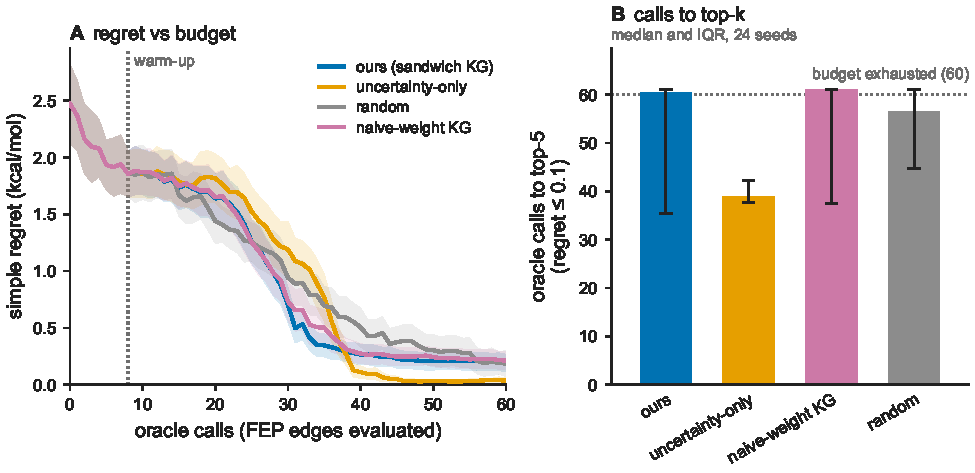
\includegraphics[width=0.78\textwidth]{figC_active_learning.pdf}
\caption{\textbf{Honest negative: edge weighting is second-order for ranking.}
The acquisition policy beats random, but the sandwich-vs-naive \emph{weighting} barely
moves calls-to-top-$k$ ($\le$$1.05\times$)---a Gauss--Markov consequence (the contrast
mean is unbiased for any positive weights).}
\label{fig:C}
\end{figure}

\begin{figure}[t]\centering
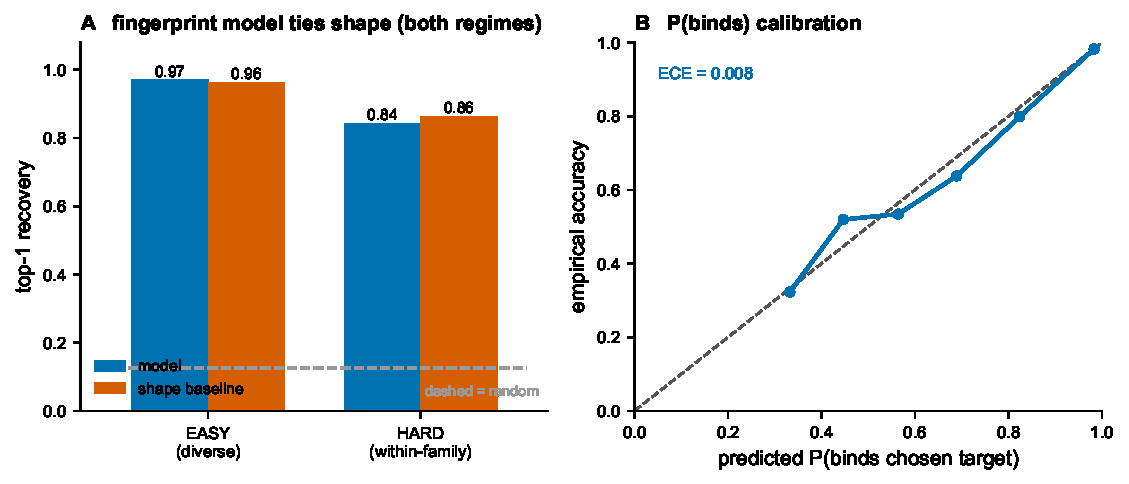
\includegraphics[width=0.92\textwidth]{figF_target_id.pdf}
\caption{\textbf{Honest case study: ligand-only reverse screening is similarity-bound.}
(A) A fingerprint model ties a Tanimoto baseline on hidden-target recovery, on both
diverse and within-family target sets. (B) $P(\text{binds})$ is well calibrated
(ECE $0.008$). Beating similarity needs orthogonal structure/physics.}
\label{fig:F}
\end{figure} The chirality and gauge results are exact and
architecture-level. We do not claim an efficiency win from edge weighting.

\section{Conclusion}
Putting a differentiable BAR estimator at the surrogate's bottleneck makes its aleatoric
uncertainty a computed, calibrated, differentiable closed form rather than a learned
guess. This readout is MBAR-correct, robust, and---because it is differentiable into a
Fisher--resistance Laplacian---usable for gauge-aware acquisition and trustworthy stopping.
Four theorems and a suite of falsifiable figures, including two honest negatives, delimit
exactly what the construction does and does not buy.

\paragraph{Reproducibility.} Every figure regenerates from one command; all theorem
constants are unit tests; real data are public (alchemtest BACE1/benzene, ChEMBL).

\end{document}
